% Created by tikzDevice version 0.12 on 2019-04-30 13:24:28
% !TEX encoding = UTF-8 Unicode
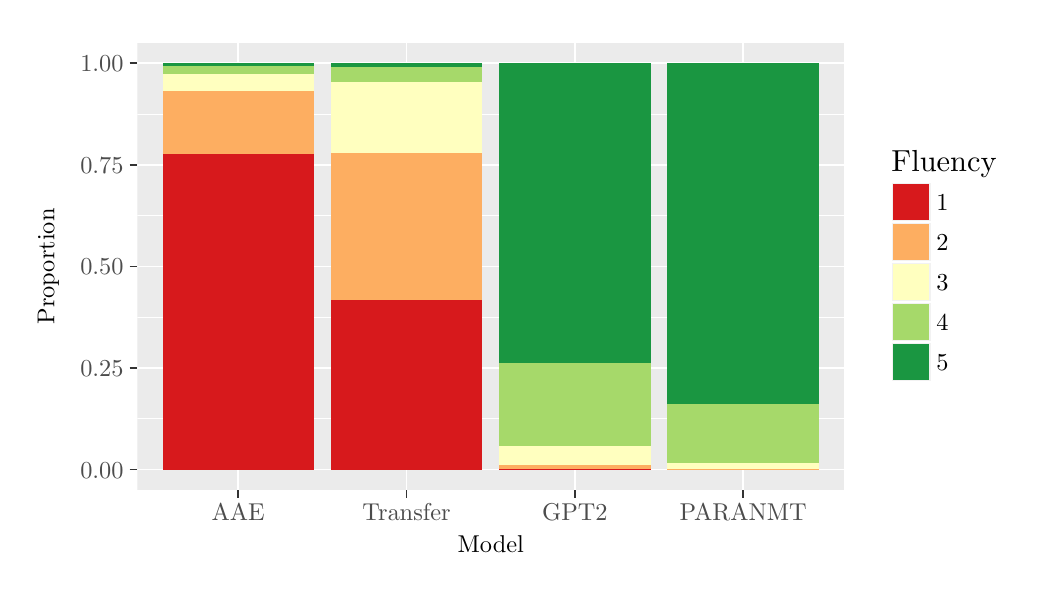
\begin{tikzpicture}[x=1pt,y=1pt]
\definecolor{fillColor}{RGB}{255,255,255}
\path[use as bounding box,fill=fillColor,fill opacity=0.00] (0,0) rectangle (361.35,195.13);
\begin{scope}
\path[clip] (  0.00,  0.00) rectangle (361.35,195.13);
\definecolor{drawColor}{RGB}{255,255,255}
\definecolor{fillColor}{RGB}{255,255,255}

\path[draw=drawColor,line width= 0.6pt,line join=round,line cap=round,fill=fillColor] (  0.00,  0.00) rectangle (361.35,195.13);
\end{scope}
\begin{scope}
\path[clip] ( 39.60, 28.07) rectangle (295.06,189.63);
\definecolor{fillColor}{gray}{0.92}

\path[fill=fillColor] ( 39.60, 28.07) rectangle (295.06,189.63);
\definecolor{drawColor}{RGB}{255,255,255}

\path[draw=drawColor,line width= 0.3pt,line join=round] ( 39.60, 53.77) --
	(295.06, 53.77);

\path[draw=drawColor,line width= 0.3pt,line join=round] ( 39.60, 90.49) --
	(295.06, 90.49);

\path[draw=drawColor,line width= 0.3pt,line join=round] ( 39.60,127.21) --
	(295.06,127.21);

\path[draw=drawColor,line width= 0.3pt,line join=round] ( 39.60,163.93) --
	(295.06,163.93);

\path[draw=drawColor,line width= 0.6pt,line join=round] ( 39.60, 35.42) --
	(295.06, 35.42);

\path[draw=drawColor,line width= 0.6pt,line join=round] ( 39.60, 72.13) --
	(295.06, 72.13);

\path[draw=drawColor,line width= 0.6pt,line join=round] ( 39.60,108.85) --
	(295.06,108.85);

\path[draw=drawColor,line width= 0.6pt,line join=round] ( 39.60,145.57) --
	(295.06,145.57);

\path[draw=drawColor,line width= 0.6pt,line join=round] ( 39.60,182.29) --
	(295.06,182.29);

\path[draw=drawColor,line width= 0.6pt,line join=round] ( 76.09, 28.07) --
	( 76.09,189.63);

\path[draw=drawColor,line width= 0.6pt,line join=round] (136.91, 28.07) --
	(136.91,189.63);

\path[draw=drawColor,line width= 0.6pt,line join=round] (197.74, 28.07) --
	(197.74,189.63);

\path[draw=drawColor,line width= 0.6pt,line join=round] (258.56, 28.07) --
	(258.56,189.63);
\definecolor{fillColor}{RGB}{215,25,28}

\path[fill=fillColor] ( 48.72, 35.42) rectangle (103.46,149.48);
\definecolor{fillColor}{RGB}{253,174,97}

\path[fill=fillColor] ( 48.72,149.48) rectangle (103.46,172.24);
\definecolor{fillColor}{RGB}{255,255,191}

\path[fill=fillColor] ( 48.72,172.24) rectangle (103.46,178.44);
\definecolor{fillColor}{RGB}{166,217,106}

\path[fill=fillColor] ( 48.72,178.44) rectangle (103.46,181.40);
\definecolor{fillColor}{RGB}{26,150,65}

\path[fill=fillColor] ( 48.72,181.40) rectangle (103.46,182.29);
\definecolor{fillColor}{RGB}{215,25,28}

\path[fill=fillColor] (109.54, 35.42) rectangle (164.28, 96.88);
\definecolor{fillColor}{RGB}{253,174,97}

\path[fill=fillColor] (109.54, 96.88) rectangle (164.28,149.78);
\definecolor{fillColor}{RGB}{255,255,191}

\path[fill=fillColor] (109.54,149.78) rectangle (164.28,175.49);
\definecolor{fillColor}{RGB}{166,217,106}

\path[fill=fillColor] (109.54,175.49) rectangle (164.28,180.81);
\definecolor{fillColor}{RGB}{26,150,65}

\path[fill=fillColor] (109.54,180.81) rectangle (164.28,182.29);
\definecolor{fillColor}{RGB}{215,25,28}

\path[fill=fillColor] (170.37, 35.42) rectangle (225.11, 35.71);
\definecolor{fillColor}{RGB}{253,174,97}

\path[fill=fillColor] (170.37, 35.71) rectangle (225.11, 37.19);
\definecolor{fillColor}{RGB}{255,255,191}

\path[fill=fillColor] (170.37, 37.19) rectangle (225.11, 43.98);
\definecolor{fillColor}{RGB}{166,217,106}

\path[fill=fillColor] (170.37, 43.98) rectangle (225.11, 73.83);
\definecolor{fillColor}{RGB}{26,150,65}

\path[fill=fillColor] (170.37, 73.83) rectangle (225.11,182.29);
\definecolor{fillColor}{RGB}{253,174,97}

\path[fill=fillColor] (231.19, 35.42) rectangle (285.93, 35.71);
\definecolor{fillColor}{RGB}{255,255,191}

\path[fill=fillColor] (231.19, 35.71) rectangle (285.93, 37.78);
\definecolor{fillColor}{RGB}{166,217,106}

\path[fill=fillColor] (231.19, 37.78) rectangle (285.93, 59.06);
\definecolor{fillColor}{RGB}{26,150,65}

\path[fill=fillColor] (231.19, 59.06) rectangle (285.93,182.29);
\end{scope}
\begin{scope}
\path[clip] (  0.00,  0.00) rectangle (361.35,195.13);
\definecolor{drawColor}{gray}{0.30}

\node[text=drawColor,anchor=base east,inner sep=0pt, outer sep=0pt, scale=  0.88] at ( 34.65, 32.38) {0.00};

\node[text=drawColor,anchor=base east,inner sep=0pt, outer sep=0pt, scale=  0.88] at ( 34.65, 69.10) {0.25};

\node[text=drawColor,anchor=base east,inner sep=0pt, outer sep=0pt, scale=  0.88] at ( 34.65,105.82) {0.50};

\node[text=drawColor,anchor=base east,inner sep=0pt, outer sep=0pt, scale=  0.88] at ( 34.65,142.54) {0.75};

\node[text=drawColor,anchor=base east,inner sep=0pt, outer sep=0pt, scale=  0.88] at ( 34.65,179.26) {1.00};
\end{scope}
\begin{scope}
\path[clip] (  0.00,  0.00) rectangle (361.35,195.13);
\definecolor{drawColor}{gray}{0.20}

\path[draw=drawColor,line width= 0.6pt,line join=round] ( 36.85, 35.42) --
	( 39.60, 35.42);

\path[draw=drawColor,line width= 0.6pt,line join=round] ( 36.85, 72.13) --
	( 39.60, 72.13);

\path[draw=drawColor,line width= 0.6pt,line join=round] ( 36.85,108.85) --
	( 39.60,108.85);

\path[draw=drawColor,line width= 0.6pt,line join=round] ( 36.85,145.57) --
	( 39.60,145.57);

\path[draw=drawColor,line width= 0.6pt,line join=round] ( 36.85,182.29) --
	( 39.60,182.29);
\end{scope}
\begin{scope}
\path[clip] (  0.00,  0.00) rectangle (361.35,195.13);
\definecolor{drawColor}{gray}{0.20}

\path[draw=drawColor,line width= 0.6pt,line join=round] ( 76.09, 25.32) --
	( 76.09, 28.07);

\path[draw=drawColor,line width= 0.6pt,line join=round] (136.91, 25.32) --
	(136.91, 28.07);

\path[draw=drawColor,line width= 0.6pt,line join=round] (197.74, 25.32) --
	(197.74, 28.07);

\path[draw=drawColor,line width= 0.6pt,line join=round] (258.56, 25.32) --
	(258.56, 28.07);
\end{scope}
\begin{scope}
\path[clip] (  0.00,  0.00) rectangle (361.35,195.13);
\definecolor{drawColor}{gray}{0.30}

\node[text=drawColor,anchor=base,inner sep=0pt, outer sep=0pt, scale=  0.88] at ( 76.09, 17.06) {AAE};

\node[text=drawColor,anchor=base,inner sep=0pt, outer sep=0pt, scale=  0.88] at (136.91, 17.06) {Transfer};

\node[text=drawColor,anchor=base,inner sep=0pt, outer sep=0pt, scale=  0.88] at (197.74, 17.06) {GPT2};

\node[text=drawColor,anchor=base,inner sep=0pt, outer sep=0pt, scale=  0.88] at (258.56, 17.06) {PARANMT};
\end{scope}
\begin{scope}
\path[clip] (  0.00,  0.00) rectangle (361.35,195.13);
\definecolor{drawColor}{RGB}{0,0,0}

\node[text=drawColor,anchor=base,inner sep=0pt, outer sep=0pt, scale=  0.88] at (167.33,  5.50) {Model};
\end{scope}
\begin{scope}
\path[clip] (  0.00,  0.00) rectangle (361.35,195.13);
\definecolor{drawColor}{RGB}{0,0,0}

\node[text=drawColor,rotate= 90.00,anchor=base,inner sep=0pt, outer sep=0pt, scale=  0.88] at (  9.62,108.85) {Proportion};
\end{scope}
\begin{scope}
\path[clip] (  0.00,  0.00) rectangle (361.35,195.13);
\definecolor{fillColor}{RGB}{255,255,255}

\path[fill=fillColor] (306.44, 61.43) rectangle (355.85,156.27);
\end{scope}
\begin{scope}
\path[clip] (  0.00,  0.00) rectangle (361.35,195.13);
\definecolor{drawColor}{RGB}{0,0,0}

\node[text=drawColor,anchor=base west,inner sep=0pt, outer sep=0pt, scale=  1.10] at (312.13,143.00) {Fluency};
\end{scope}
\begin{scope}
\path[clip] (  0.00,  0.00) rectangle (361.35,195.13);
\definecolor{drawColor}{RGB}{255,255,255}
\definecolor{fillColor}{gray}{0.95}

\path[draw=drawColor,line width= 0.6pt,line join=round,line cap=round,fill=fillColor] (312.13,124.94) rectangle (326.58,139.39);
\end{scope}
\begin{scope}
\path[clip] (  0.00,  0.00) rectangle (361.35,195.13);
\definecolor{fillColor}{RGB}{215,25,28}

\path[fill=fillColor] (312.84,125.65) rectangle (325.87,138.68);
\end{scope}
\begin{scope}
\path[clip] (  0.00,  0.00) rectangle (361.35,195.13);
\definecolor{drawColor}{RGB}{255,255,255}
\definecolor{fillColor}{gray}{0.95}

\path[draw=drawColor,line width= 0.6pt,line join=round,line cap=round,fill=fillColor] (312.13,110.48) rectangle (326.58,124.94);
\end{scope}
\begin{scope}
\path[clip] (  0.00,  0.00) rectangle (361.35,195.13);
\definecolor{fillColor}{RGB}{253,174,97}

\path[fill=fillColor] (312.84,111.19) rectangle (325.87,124.23);
\end{scope}
\begin{scope}
\path[clip] (  0.00,  0.00) rectangle (361.35,195.13);
\definecolor{drawColor}{RGB}{255,255,255}
\definecolor{fillColor}{gray}{0.95}

\path[draw=drawColor,line width= 0.6pt,line join=round,line cap=round,fill=fillColor] (312.13, 96.03) rectangle (326.58,110.48);
\end{scope}
\begin{scope}
\path[clip] (  0.00,  0.00) rectangle (361.35,195.13);
\definecolor{fillColor}{RGB}{255,255,191}

\path[fill=fillColor] (312.84, 96.74) rectangle (325.87,109.77);
\end{scope}
\begin{scope}
\path[clip] (  0.00,  0.00) rectangle (361.35,195.13);
\definecolor{drawColor}{RGB}{255,255,255}
\definecolor{fillColor}{gray}{0.95}

\path[draw=drawColor,line width= 0.6pt,line join=round,line cap=round,fill=fillColor] (312.13, 81.57) rectangle (326.58, 96.03);
\end{scope}
\begin{scope}
\path[clip] (  0.00,  0.00) rectangle (361.35,195.13);
\definecolor{fillColor}{RGB}{166,217,106}

\path[fill=fillColor] (312.84, 82.29) rectangle (325.87, 95.32);
\end{scope}
\begin{scope}
\path[clip] (  0.00,  0.00) rectangle (361.35,195.13);
\definecolor{drawColor}{RGB}{255,255,255}
\definecolor{fillColor}{gray}{0.95}

\path[draw=drawColor,line width= 0.6pt,line join=round,line cap=round,fill=fillColor] (312.13, 67.12) rectangle (326.58, 81.57);
\end{scope}
\begin{scope}
\path[clip] (  0.00,  0.00) rectangle (361.35,195.13);
\definecolor{fillColor}{RGB}{26,150,65}

\path[fill=fillColor] (312.84, 67.83) rectangle (325.87, 80.86);
\end{scope}
\begin{scope}
\path[clip] (  0.00,  0.00) rectangle (361.35,195.13);
\definecolor{drawColor}{RGB}{0,0,0}

\node[text=drawColor,anchor=base west,inner sep=0pt, outer sep=0pt, scale=  0.88] at (328.39,129.13) {1};
\end{scope}
\begin{scope}
\path[clip] (  0.00,  0.00) rectangle (361.35,195.13);
\definecolor{drawColor}{RGB}{0,0,0}

\node[text=drawColor,anchor=base west,inner sep=0pt, outer sep=0pt, scale=  0.88] at (328.39,114.68) {2};
\end{scope}
\begin{scope}
\path[clip] (  0.00,  0.00) rectangle (361.35,195.13);
\definecolor{drawColor}{RGB}{0,0,0}

\node[text=drawColor,anchor=base west,inner sep=0pt, outer sep=0pt, scale=  0.88] at (328.39,100.23) {3};
\end{scope}
\begin{scope}
\path[clip] (  0.00,  0.00) rectangle (361.35,195.13);
\definecolor{drawColor}{RGB}{0,0,0}

\node[text=drawColor,anchor=base west,inner sep=0pt, outer sep=0pt, scale=  0.88] at (328.39, 85.77) {4};
\end{scope}
\begin{scope}
\path[clip] (  0.00,  0.00) rectangle (361.35,195.13);
\definecolor{drawColor}{RGB}{0,0,0}

\node[text=drawColor,anchor=base west,inner sep=0pt, outer sep=0pt, scale=  0.88] at (328.39, 71.32) {5};
\end{scope}
\end{tikzpicture}
